\newpage
\section{Νευρωνικά Δίκτυα}
Τα νευρωνικά δίκτυα είναι στις μέρες μας το κυρίαρχο μοντέλο στη μηχανική μάθηση και μπορεί να λύσει και τους τρεις τύπους προβλημάτων που έχουμε δει (ταξινόμηση, παλινδρόμηση και ομαδοποίηση). Τα τεχνητά νευρωνικά δίκτυα δημιουργήθηκαν με
σκοπό να μιμηθούν τον τρόπο που λειτουργεί ο εγκέφαλος του ανθρώπου. Οι νευρώνες του εγκεφάλου μας λειτουργούν δημιουργώντας συνδέσεις με άλλους νευρώνες και όλοι μαζί συμβάλουν στην επεξεργασία ενός ηλεκτρικού σήματος που έρχεται από τον
εγκέφαλο το οποίο τελικά καταλήγει να είναι απλή καθημερινή πράξη για τον άνθρωπο (όπως για παράδειγμα να κουνήσει το χέρι του)\cite{nnip}.

Τα τεχνητά νευρωνικά δίκτυα προσπαθούν λοιπόν να αντιγράψουν αυτη ακριβώς την ιδιότητα. Ο σκοπός τους είναι να παίρνουν μια είσοδο και να παράγουν μία απάντηση. Για παράδειγμα θα μπορούσαμε σαν είσοδο να δώσουμε τις αιματολογικές εξετάσεις
ενός ανθρώπου και η έξοδος να είναι 0 ή 1 ανάλογα αν έχει μια ασθένεια ή όχι. Αυτό είναι ένα πρόβλημα δυαδικής ταξινόμησης αλλά θα μπορούσαμε να λύσουμε και πολλά άλλα προβλήματα και θα αναλύσουμε στην συνέχεια τις αλλαγές που πρέπει να
κάνουμε σε ένα νευρωνικό δίκτυο ανάλογα το πρόβλημα. Σε αυτή την ενότητα θα αναλύσουμε διάφορες έννοιες τις οποίες πρέπει να γνωρίζει κανείς αν θέλει να κατανοήσει τα νευρωνικά δίκτυα. Αυτές είναι\cite{nnav}:
\begin{itemize}
    \item Νευρώνας
    \item Επίπεδο
    \item Οπισθοδρόμηση (\en{back propagation})
    \item Συναρτήσεις ενεργοποίησης
    \item Συναρτήσεις σφάλματος
\end{itemize}

\subsection{Νευρώνας}
\subsection{Επίπεδο}
\subsection{Οπισθοδρόμηση}
\subsection{Συναρτήσεις ενεργοποίησης}
Οι συναρτήσεις ενεργοποίησης είναι ένα πολύ σημαντικό κομμάτι των νευρωνικών δικτύων διότι προσφέρουν μη γραμμικότητα (επιθυμητή) στο σύστημά μας. Για να καταλάβουμε καλύτερα τι σημαίνει αυτό θα δούμε ένα παράδειγμα\cite{nnactmlm}:

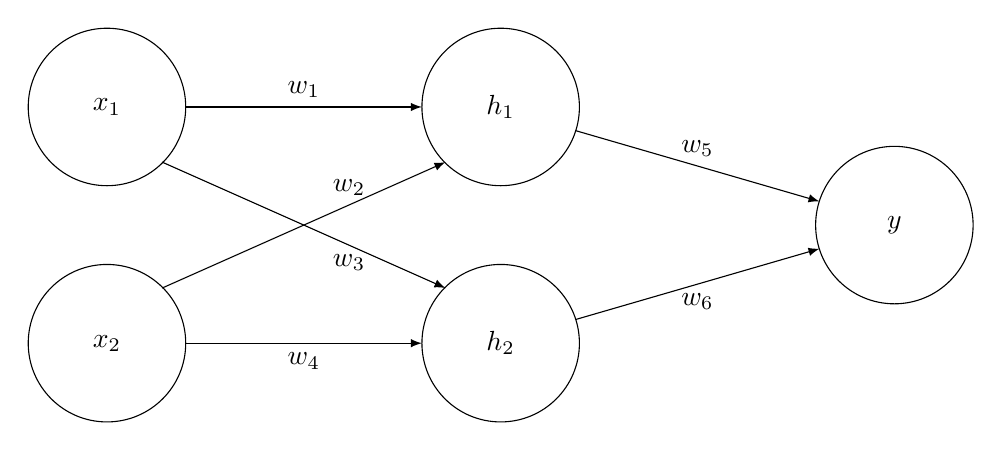
\begin{tikzpicture}
    \draw (0,0) circle (1) node{$x_2$};
    \draw (0,3) circle (1) node{$x_1$};
    \draw (5,0) circle (1) node{$h_2$};
    \draw (5,3) circle (1) node{$h_1$};
    \draw (10,1.5) circle (1) node{$y$};

    \draw[-latex] (1,0) -- (4,0) node[midway, below]{$w_4$};
    \draw[-latex] (1,3) -- (4,3) node[midway, above]{$w_1$};

    \draw[-latex] (0.7,0.7) -- (4.3,2.3) node[midway, above right=7]{$w_2$};
    \draw[-latex] (0.7,2.3) -- (4.3,0.7) node[midway, below right=7]{$w_3$};

    \draw[-latex] (5.95,2.7) -- (9.05,1.8) node[midway, above]{$w_5$};
    \draw[-latex] (5.95,0.3) -- (9.05,1.2) node[midway, below]{$w_6$};
\end{tikzpicture}

Βλεπουμε ότι η είσοδος με την έξοδο συνδέονται μέσω ενός κρυφού επιπέδου (\en{dense}) όπου:
\begin{gather*}
    h_1=w_1\times x_1+w_2\times x_2 \\
    h_2=w_3\times x_1+w_4\times x_2 \\
    y=w_5\times h_1+w_6\times h_2 \\
\end{gather*}
Αν αναλύσουμε λοιπόν τον τύπο του $y$ θα πάρουμε:
$$y=w_1(w_5\times x_1+w_2\times x_2) + w_6(w_3\times x_1+w_4\times x_2)$$
Που τελικά γίνεται:
$$y=(w_1w_5+w_3w_6)\times x_1+(w_2w_5+w_4w_6)\times x_2$$
Τα $w$ είναι σταθεροί αριθμοί οπότε τελικά ενώ έχουμε ένα κρυφό επίπεδο ανάμεσα στην είσοδο και στην έξοδο αυτές συνδέονται και πάλι με γραμμική σχέση. Το ίδιο θα συνέβαινε και για πολλαπλά κρυφά επίπεδα με πολλούς νευρώνες. Αυτό για το
δίκτυο μας σημαίνει ότι μπορεί να προσεγγίσει δεδομένα που ακολουθούν επίσης μια γραμμική σχέση. Τα δεδομένα όμως συνήθως δεν έχουν τέτοια συμπεριφορά. Για να λύσουμε αυτό το πρόβλημα δημιουργήθηκαν οι συναρτήσεις ενεργοποίησης. Στο
παράδειγμά μας μπορούμε να προσθέσουμε μις συνάρτηση ενεργοποίησης αμέσως μετά το κρυφό επίπεδο. Έτσι τελικά η έξοδος θα είναι:
$$y=w_5\times f_A(h_1)+w_6\times f_A(h_2)$$
Όπου $f_A$ η συνάρτηση ενεργοποίησης. Παρατηρούμε ότι η είσοδος δεν μπορεί πλέον να συνδεθεί γραμμικά με την έξοδο και άρα έχουμε πετύχει τον στόχο μας.

Υπάρχουν πολλές συναρτήσεις ενεργοποίησης και όλες έχουν τα πλεονεκτήματα και τα μειονεκτήματα τους. Εμεις θα αναλύσουμε κάποιες από τις πιο γνωστές οι οποίες χρησιμοποιούνται σχεδόν πάντα στα νευρωνικά δίκτυα.
Από τις πρώτες συναρτήσεις ενεργοποίησης ήταν η βηματική συνάρτηση:
\[f(x)=\left\{\begin{array}{ll}0 & x<0 \\ 1 & x>=0 \\ \end{array} \right.\]
\begin{figure}[H]
    \centering
    \begin{tikzpicture}
    \begin{axis}[axis lines=middle, xlabel=$x$, ylabel=$y$, xmin = -5, xmax=5, ymin=0, ymax=2, xtick={-5,-4,...,5}, ytick={0,1,2}]
        \addplot[color=red, domain=0:10]{1};
        \addplot[color=red, domain=-10:0]{0};
    \end{axis}
    \end{tikzpicture}
    \caption{\en{step function}}
\end{figure}
Η βηματική συνάρτηση είναι χρήσιμη όταν έχουμε ένα πρόβλημα δυαδικής ταξινόμησης. Μπορούμε δηλαδή να την εφαρμόσουμε στο επίπεδο εξόδου έτσι ώστε η απάντηση που θα παίρνουμε να είναι πάντα  0 ή 1. Όμως έχει ένα μεγάλο μειονέκτημά το οποίο
είναι ότι δεν είναι συνεχής. Η τεχνική της Οπισθοδρόμησης βασίζεται στις παραγώγους των συναρτήσεων κάτι το οποίο την κάνει πολύ δύσχρηστη. Θα μπορούσαμε θεωρητικά να αγνοήσουμε το 0 στο οποίο η συνάρτηση δεν είναι παραγωγίσιμη και να του
δώσουμε μια τιμή (όπως 0) αλλά υπάρχει ένα ακόμα πρόβλημα. Το πρόβλημα είναι ότι η παράγωγός της είναι παντού 0 και γνωρίζουμε από την οπισθοδρόμηση ότι πρέπει να πολλαπλασιάσουμε το σφάλμα με αυτή την παράγωγο. Άρα τελικά το σφάλμα που θα διαδίδεται στα επίπεδα θα είναι μηδενικό και άρα δεν θα γίνεται καμία διόρθωση.

Μια καλύτερη συνάρτηση που διατηρεί τα χαρακτηριστικά της βηματικής είναι η σιγμοειδής:
$$f(x)=\frac{1}{1+e^{-x}}$$
\begin{figure}[H]
    \centering
    \begin{tikzpicture}
    \begin{axis}[axis lines=middle, xlabel=$x$, ylabel=$y$, xmin = -5, xmax=5, ymin=0, ymax=2, xtick={-5,-4,...,5}, ytick={0,1,2}]
        \addplot[color=red]{exp(x)/(exp(x)+1)};
    \end{axis}
    \end{tikzpicture}
    \caption{\en{sigmoid function}}
\end{figure}
Αυτή η συνάρτηση είναι επίσης φραγμένη από το 0 ως το 1 και για αυτό μπορεί να χρησιμοποιηθεί επίσης στο επίπεδο εξόδου για δυαδική ταξινόμηση. Η σιγμοειδής όμως έχει ποιο ομαλή και συνεχή μετάβαση από το 0 στο 1 άρα μπορούμε να εφαρμόσουμε
τους κανόνες της οπισθοδρόμησης. Χρησιμοποιείται λοιπόν με αυτόν τον τρόπο μέχρι και σήμερα. Παρ' όλα αυτά για τα κρυφά επίπεδα, τα οποία δεν είναι απαραίτητο να κυμαίνονται απο 0 μέχρι 1, υπάρχει μια ακόμα καλύτερη συνάρτηση. Αυτή είναι η
συνάρτηση της υπερβολικής εφαπτομένης:
$$f(x)=\tanh (x)=\frac{e^x-e^{-x}}{e^x+e^{-x}}$$
\begin{figure}[H]
    \centering
    \begin{tikzpicture}
    \begin{axis}[axis lines=middle, xlabel=$x$, ylabel=$y$, xmin = -5, xmax=5, ymin=-2, ymax=2, xtick={-5,-4,...,5}, ytick={-2,-1,...,2}]
        \addplot[color=red]{tanh(x)};
    \end{axis}
    \end{tikzpicture}
    \caption{\en{tanh function}}
\end{figure}
Η συνάρτηση αυτή είναι καλύτερη επειδή αντιμετωπίζει το λεγόμενο \en{vanishing gradient problem}. Για να καταλάβουμε τι σημαίνει αυτό θα πρέπει να συγκρίνουμε τις παραγώγους των δύο συναρτήσεων:
\begin{figure}[H]
    \centering
    \begin{subfigure}{0.49\textwidth}
        \centering
        \begin{tikzpicture}
        \begin{axis}[axis lines=middle, xlabel=$x$, ylabel=$y$, xmin = -5, xmax=5, ymin=0, ymax=1, xtick={-5,-4,...,5}, ytick={0,0.25,...,1}]
            \addplot[color=red]{(exp(x)/(exp(x)+1))*(1-(exp(x)/(exp(x)+1)))};
        \end{axis}
        \end{tikzpicture}
        \caption{\en{sigmoid derivative}}
    \end{subfigure}
    \begin{subfigure}{0.49\textwidth}
        \centering
        \begin{tikzpicture}
        \begin{axis}[axis lines=middle, xlabel=$x$, ylabel=$y$, xmin = -5, xmax=5, ymin=0, ymax=1, xtick={-5,-4,...,5}, ytick={0,0.25,...,1}]
            \addplot[color=red]{1-tanh(x)^2};
        \end{axis}
        \end{tikzpicture}
        \caption{\en{tanh derivative}}
    \end{subfigure}
    \caption{\en{derivative comparison}}
\end{figure}
Από το παραπάνω σχήμα μπορούμε να δούμε ότι η παράγωγός της σιγμοειδούς έχει μέγιστη τιμή το 0.25. Αυτό σημαίνει ότι αν έχουμε πολλά κρυφά επίπεδα με αυτή την ενεργοποίηση, κάθε φορά που το σφάλμα θα διαδίδεται από το ένα επίπεδο στο άλλο
θα υπο-τετραπλασιάζεται στην καλύτερη περίπτωση. Έτσι στο τέλος τα αρχικά επίπεδα θα κάνουν ελάχιστη διόρθωση στα βάρη τους. Αντιθέτως η παράγωγος της υπερβολικής εφαπτομένης έχει μέγιστο το 1 άρα δίνει πολύ καλύτερα αποτελέσματα. Παρ' ότι
μειώνεται το πρόβλημα όμως δεν εξαφανίζεται. Γι' αυτό οι επόμενες συναρτήσεις που θα δούμε αντιμετωπίζουν πλήρως το \en{vanishing gradient problem}.

Η επόμενη συνάρτηση που αυτή τη στιγμή είναι και η πιο διάσημη συνάρτηση ενεργοποίησης στη μηχανική μάθηση είναι η \en{ReLU (rectified linear unit)}:
\[f(x)=\left\{\begin{array}{ll}0 & x<0 \\ x & x>=0 \\ \end{array} \right.\]
\begin{figure}[H]
    \centering
    \begin{tikzpicture}
    \begin{axis}[axis lines=middle, xlabel=$x$, ylabel=$y$, xmin = -5, xmax=5, ymin=0, ymax=5, xtick={-5,-4,...,5}, ytick={0,1,...,5}, axis equal]
        \addplot[color=red, domain=0:10]{x};
        \addplot[color=red, domain=-10:0]{0};
    \end{axis}
    \end{tikzpicture}
    \caption{\en{ReLU function}}
\end{figure}
Η συνάρτηση αυτή έχει την ικανότητα να προσφέρει ταυτόχρονα τα πλεονεκτήματα της γραμμικότητας αλλά και της μη γραμμικότητας. Λόγω της γραμμικότητας δεν έχει το \en{vanishing gradient problem} και επίσης έχει πολύ απλή υλοποίηση. Αλλά η μη
γραμμικότητα που έχει της επιτρέπει να εφαρμόζει την επιθυμητή μη γραμμικότητα που θέλουμε στα νευρωνικά δίκτυα. Ενώ η συνάρτηση είναι η πιο διάσημη δεν σημαίνει ότι δεν έχει και αυτή τα προβλήματά της. Συγκεκριμένα μιλάμε για το λεγόμενο
\en{dying ReLU problem}. Συγκεκριμένα η παράγωγός της για αρνητικές τιμές είναι 0. Αυτό σημαίνει ότι όταν είναι αρνητική η είσοδος δεν θα μπορεί να διαδοθεί το σφάλμα από εκείνο το επίπεδο. Γι' αυτό και οι επόμενες συναρτήσεις που θα δούμε
είναι παραλλαγές αυτής της συνάρτησης με σκοπό να αντιμετωπίσουν αυτό το πρόβλημα. Ξεκινάμε με την \en{Leaky ReLU}:
\[f(x)=\left\{\begin{array}{ll}0.01x & x<0 \\ x & x>=0 \\ \end{array} \right.\]
\begin{figure}[H]
    \centering
    \begin{tikzpicture}
    \begin{axis}[axis lines=middle, xlabel=$x$, ylabel=$y$, xmin = -5, xmax=5, ymin=0, ymax=5, xtick={-5,-4,...,5}, ytick={0,1,...,5}, axis equal]
        \addplot[color=red, domain=0:10]{x};
        \addplot[color=red, domain=-10:0]{0.1*x};
    \end{axis}
    \end{tikzpicture}
    \caption{\en{ReLU function}}
\end{figure}
Γενίκευση της αποτελει τη \en{parametric ReLU} με τύπο:
\[f(x)=\left\{\begin{array}{ll}ax & x<0 \\ x & x>=0 \\ \end{array} \right.\]
Αυτές αντιμετωπίζουν το πρόβλημα με έναν πολύ απλό τρόπο. Παρ' όλα αυτά έχουν βρεθεί και πιο πολύπλοκες συναρτήσεις που θα δούμε παρακάτω. Ακολουθεί η συνάρτηση \en{ELU (exponential linear unit)}:
\[f(x)=\left\{\begin{array}{ll}a(e^x-1) & x<0 \\ x & x>=0 \\ \end{array} \right.\]
\begin{figure}[H]
    \centering
    \begin{tikzpicture}
    \begin{axis}[axis lines=middle, xlabel=$x$, ylabel=$y$, xmin = -5, xmax=5, ymin=0, ymax=5, xtick={-5,-4,...,5}, ytick={0,1,...,5}, axis equal]
        \addplot[color=red, domain=0:10]{x};
        \addplot[color=red, domain=-10:0]{(exp(x)-1)};
    \end{axis}
    \end{tikzpicture}
    \caption{\en{ELU function}}
\end{figure}
Όπως και πριν μπορούμε να γενικεύσουμε αυτή τη συνάρτηση. Η γενικευμένη μορφή ονομάζεται \en{SELU (scaled exponential linear unit)}:
\[f(x)=\lambda\left\{\begin{array}{ll}a(e^x-1) & x<0 \\ x & x>=0 \\ \end{array} \right.\]
\begin{figure}[H]
    \centering
    \begin{tikzpicture}
    \begin{axis}[axis lines=middle, xlabel=$x$, ylabel=$y$, xmin = -5, xmax=5, ymin=-5, ymax=5, xtick={-5,-4,...,5}, ytick={0,1,...,5}, axis equal]
        \addplot[color=red, domain=0:10]{x};
        \addplot[color=red, domain=-10:0]{2*(exp(x)-1)};
    \end{axis}
    \end{tikzpicture}
    \caption{\en{SELU function}}
\end{figure}
Οι παραπάνω συναρτήσεις όπως έχουμε δει έχουν δύο κλάδους με σκοπό να πετύχουν τη γραμμικά και μη γραμμικά στοιχεία που θέλουμε. Οι παρακάτω συναρτήσεις καταφέρνουν να έχουν παρόμοια συμπεριφορά με έναν τύπο συνάρτησης. Η μία από αυτές
είναι η \en{GELU (Gaussian error linear unit)}:
$$0.5x\left(1+\tanh \left[\frac{\sqrt{2}}{\pi}(x+0.044715x^3)\right]\right)$$
\begin{figure}[H]
    \centering
    \begin{tikzpicture}
    \begin{axis}[axis lines=middle, xlabel=$x$, ylabel=$y$, xmin = -5, xmax=5, ymin=0, ymax=5, xtick={-5,-4,...,5}, ytick={0,1,...,5}, axis equal]
        \addplot[color=red]{0.5*x*(1+tanh(sqrt(2)/pi*(x+0.044715*x^3)))};
    \end{axis}
    \end{tikzpicture}
    \caption{\en{GELU function}}
\end{figure}




\begin{tikzpicture}
\begin{axis}[axis lines=middle, xlabel=$x$, ylabel=$y$, title=\en{swish function}, xmin = -5, xmax=5, ymin=-2, ymax=2, xtick={-5,-4,...,5}, ytick={0,1,2}, axis equal]
    \addplot[color=red]{x/(exp(-x)+1)};
\end{axis}
\end{tikzpicture}


\subsection{Συναρτήσεις σφάλματος}